\documentclass[12pt]{article}
\usepackage{amsmath}
\usepackage{amssymb}
\usepackage[letterpaper,top=1.2in,bottom=1in,left=0.75in,right=0.75in,centering]{geometry}
%\usepackage{fancyhdr}
\usepackage{enumerate}
%\usepackage{lastpage}
\usepackage{multicol}
\usepackage{graphicx}

\reversemarginpar

%\pagestyle{fancy}
%\cfoot{}
%\lhead{Math 1560}\chead{Test \# 1}\rhead{May 18th, 2017}
%\rfoot{Total: 10 points}
%\chead{{\bf Name:}}
\newcommand{\points}[1]{\marginpar{\hspace{24pt}[#1]}}
\newcommand{\skipline}{\vspace{12pt}}
%\renewcommand{\headrulewidth}{0in}
\headheight 30pt

\newcommand{\di}{\displaystyle}
\newcommand{\abs}[1]{\lvert #1\rvert}
\newcommand{\len}[1]{\lVert #1\rVert}
\renewcommand{\i}{\mathbf{i}}
\renewcommand{\j}{\mathbf{j}}
\renewcommand{\k}{\mathbf{k}}
\newcommand{\R}{\mathbb{R}}
\newcommand{\aaa}{\mathbf{a}}
\newcommand{\bbb}{\mathbf{b}}
\newcommand{\ccc}{\mathbf{c}}
\newcommand{\dotp}{\boldsymbol{\cdot}}
\newcommand{\bbm}{\begin{bmatrix}}
\newcommand{\ebm}{\end{bmatrix}}       
\newcommand{\bvm}{\begin{vmatrix}}
\newcommand{\evm}{\end{vmatrix}}       
\DeclareMathOperator{\proj}{proj}            
                  
\begin{document}


\author{Instructor: Sean Fitzpatrick}
\thispagestyle{empty}
\vglue1cm
\begin{center}
{\bf MATH 1410 - Tutorial \#5 Solutions}
\end{center}




%\newpage
%\thispagestyle{empty}

\textbf{Assigned problems:}
\begin{enumerate}

  
 \item Find the equation of the plane that contains the point $P=(-2,0,5)$ and the line\\ $\langle x,y,z\rangle = \langle 5-3t,2-t,-4+5t\rangle$.


\bigskip

We know that one vector parallel to the plane is the direction vector $\vec{v}=\langle -3,-1,5\rangle$ for the line. To obtain another, note that the point $P=(-2,0,5)$ is on the plane, and to get a second point, we can take any point on the line; for example, the point $Q=(5,2,-4)$ obtained by setting $t=0$. We then get the vector
\[
\vec{w}=\overrightarrow{PQ}=\langle 7,2,-9\rangle,
\]
which is also parallel to the plane. A normal vector is then
\[
\vec{n}=\vec{v}\times\vec{w} = \bvm \i&\j&\k\\-3&-1&5\\7&2&-9\evm = \langle -1, 8, 1\rangle,
\]
and an equation for the plane is given by
\[
-1(x+2)+8y+(z-5)=0.
\]

\item Determine the equation of the line of intersection of the planes $x-3y+2z=4$\\ and $-2x+4y-3z=-3$.

The line of intersection consists of all points $(x,y,z)$ that satisfy the equations of both planes. That is, we are looking for all $x,y,z$ that satisfy the \textit{system}
\[\arraycolsep1pt
\begin{array}{ccccccc}
x&-&3y&+&2z&=&4\\
-2x&+&4y&-&3z&=&-3
\end{array}
\]
To find our line, we attempt to simplify the above system. Adding twice the first equation to the second, we eliminate $x$ from the second equation, giving us
\[\arraycolsep1pt
\begin{array}{ccccccc}
x&-&3y&+&2z&=&4\\
& &-2y&+&z&=&5
\end{array}
\]
We can now eliminate $z$ in the second equation by subtracting twice the second equation from the first\footnote{\textbf{Caution:} this is not the standard algorithm you'll encounter after the break. Normally we'd eliminate $y$ from the first equation, but we're breaking with convention here to avoid fractions and an extra step.}
\[\arraycolsep1pt
\begin{array}{ccccccc}
x&+&y&&&=&-6\\
& &-2y&+&z&=&5
\end{array}
\]
 We now solve the first equation for $x$, giving us $x=-6-y$, and the second for $z$, giving us $z=5+2y$. If we let $y=t$ be an independent parameter, then we obtain the parametric equations
 \begin{align*}
 x&=-6-t\\
 y&=t\\
 z&=5+2t
 \end{align*}
 or the vector equation $\langle x,y,z\rangle = \langle -6,0,5\rangle +t\langle -1,1,2\rangle$.
 
 (By the way, note that the direction vector for this line is indeed orthogonal to the normal vectors of the two planes, as we should expect.)
 
 \bigskip
 
 Alternative solution: another way to solve this is to note that the direction vector for the line must be orthogonal to the normal vectors for the two planes, so we can obtain a direction vector by computing the cross product of the two normal vectors:
 \[
 \vec{n} = \langle 1,-3,2\rangle\times\langle -2,4,-3\rangle = \langle 1, -1,-2\rangle.
 \]
 Note that this is just the negative of the one we found above.
 
 Next we need a point on the line. If we set $z=0$ in the equations for both planes (there is no particular reason for this choice other than the need to eliminate one variable), we get the system of two equations in two variables given by
 \[\arraycolsep1pt
\begin{array}{ccccc}
x&-&3y&=&4\\
-2x&+&4y&=&-3
\end{array}
\]
We can solve this using techniques similar to the above. Adding twice the first equation to the second gives simply $-2y=5$, so $y=-5/2$. Putting this back into the first equation gives $x=4+3(-5/2)=-7/2$.

Thus, we have the point $(-7/2,-5/2,0)$ on our line, so the vector equation of the line is
\[
\langle x,y,z\rangle = \langle -\frac72,-\frac52,0\rangle + t\langle 1,-1,-2\rangle.
\]
Note that putting $t=-5/2$ gives the point $(-6,0,5)$ that we had found using the other method above.

\pagebreak

\item Find the point $Q$ on the plane $x-2y-2z=1$ that is closest the point $P=(2,8,5)$, and the distance from $P$ to the plane,
\begin{enumerate}
\item Using vector projections.\\
{\em Hint:} Begin by finding any point $P_0$ that lies on the plane. {\bf Include a diagram.}

\bigskip

\begin{multicols}{2}
We first choose a point on the plane $x-2y-2z=1$. If we set $y=z=0$ in this equation, we're left with $x=1$, so we can take $P_0=(1,0,0)$.  
\columnbreak

\begin{center}
 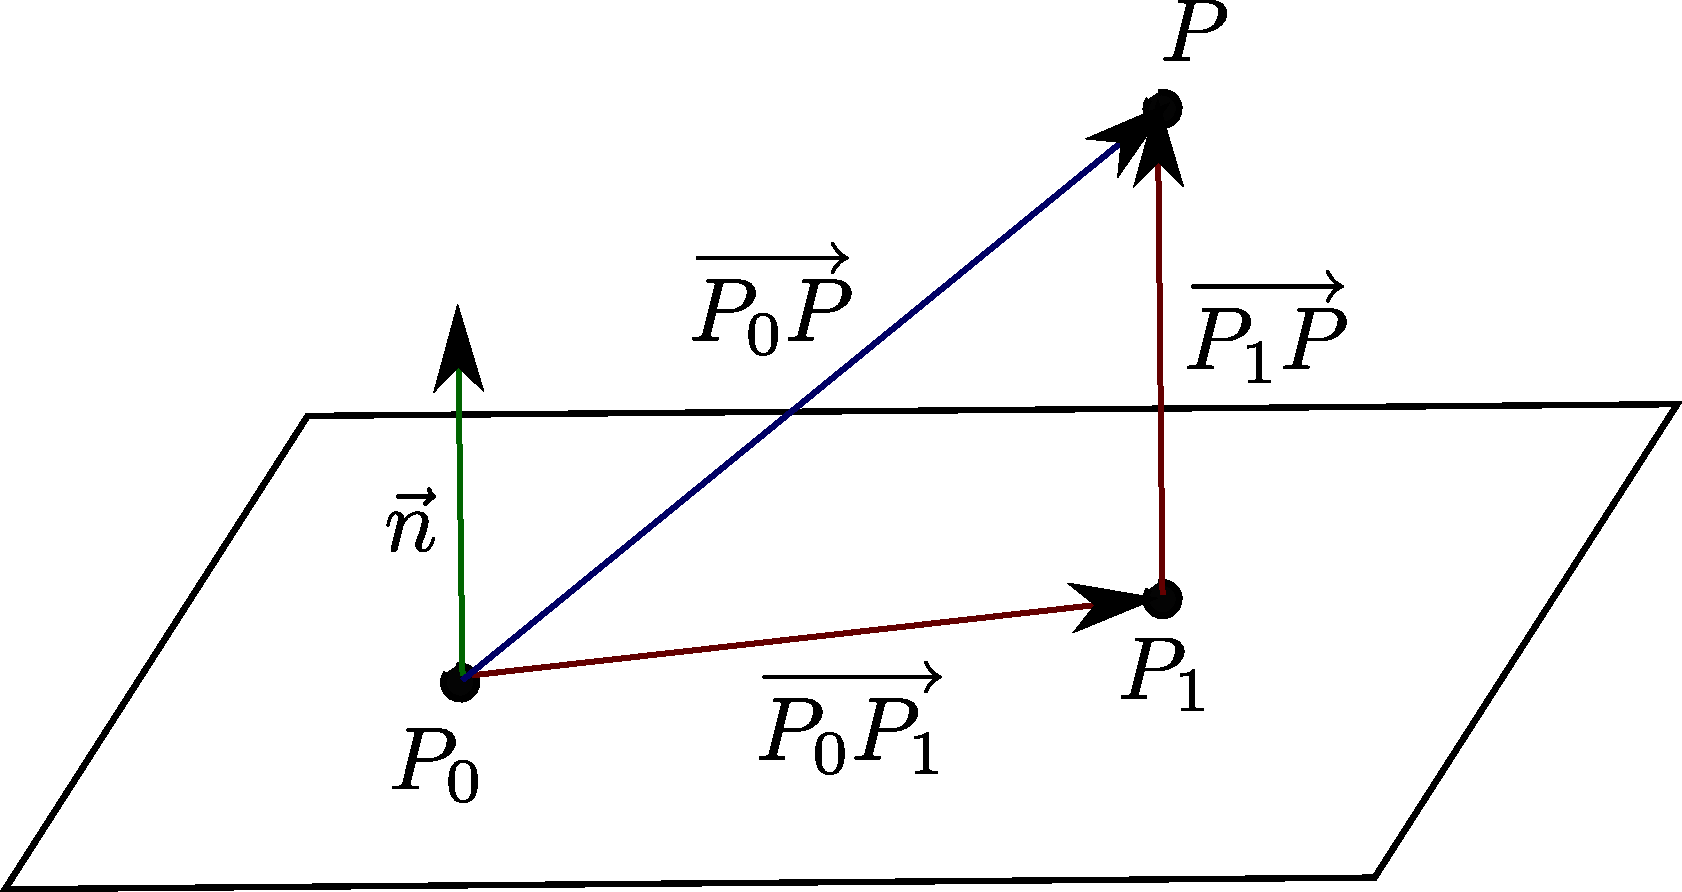
\includegraphics[width=0.8\columnwidth]{WS3-4}
\end{center}
\end{multicols}
Now, referring to the diagram above, we see that the desired distance is given by the length of the vector $\overrightarrow{P_1P}$, where $P_1$ is the point on the plane closest to $P$. Moreover, this vector is the projection of the vector $\overrightarrow{P_0P}$ onto the normal vector $\vec{n}$: $\overrightarrow{P_1P} = \proj_{\vec{n}}\overrightarrow{P_0P}$. (Your answer will not depend on the point $P_0$ that you choose. Changing $P_0$ will change the vectors $\overrightarrow{P_0}$ and $\overrightarrow{P_0P_1}$, but it will not change the vector $\overrightarrow{P_1P}$.)

Recalling that for a general plane $ax+by+cz=d$, the normal vector is given by $\vec{n} = \langle a, b, c\rangle$, we conclude from the equation $x-2y-2z=1$ that our normal vector is $\vec{n} = \langle 1, -2, -2\rangle$. Since we chose $P_0=(1,0,0)$, we have
\[
 \overrightarrow{P_0P} = \overrightarrow{OP}-\overrightarrow{OP_0} = \langle 2, 8, 5\rangle - \langle 1, 0, 0\rangle = \langle 1, 8, 5\rangle.
\]
Since $\vec{n}\dotp\overrightarrow{P_0P} = 1(1)-2(8)-2(5) = -25$ and $\len{\vec{n}} = \sqrt{1^2+(-2)^2+(-2)^2} = \sqrt{9}=3$, we have
\[
 \overrightarrow{P_1P} = \proj_{\vec{n}}\overrightarrow{P_0P} = \left(\frac{\vec{n}\dotp\overrightarrow{P_0P}}{\len{\vec{n}}^2}\right)\vec{n} = \left(\frac{-25}{9}\right)\langle 1, -2, -2\rangle = \langle -25/9, 50/9, 50/9\rangle.
\]
The distance from $P$ to the plane is therefore
\[
 d=\len{\overrightarrow{P_1P}} = \left\lVert \left(\frac{-25}{9}\right)\langle 1, -2, -2\rangle\right\rVert = \frac{25}{9}\left\lVert \langle 1, -2, -2\rangle\right\rVert = \frac{25}{9}(3) = \frac{25}{3}.
\]
To find the point $P_1$, we note that $\overrightarrow{P_1P} = \overrightarrow{OP}-\overrightarrow{OP_1}$, so
\begin{align*}
 \overrightarrow{OP_1} = \overrightarrow{OP}-\overrightarrow{P_1P} &= \langle 2, 8, 5\rangle - \left\langle -\frac{25}{9}, \frac{50}{9}, \frac{50}{9}\right\rangle\\
& = \left\langle 2+\frac{25}{9}, 8-\frac{50}{9}, 5-\frac{50}{9}\right\rangle = \left\langle \frac{43}{9}, \frac{22}{9}, -\frac{5}{9}\right\rangle,
\end{align*}
so $P_1 = \left(\dfrac{43}{9},\dfrac{22}{9},-\dfrac{5}{9}\right)$.




\item By finding where the line through $P$ in the direction perpendicular to the plane intersects the plane.

\bigskip

Referring again to the diagram above, if we construct the line $L$ that passes through the point $P$ in the direction of the normal vector $\vec{n}$, then the point $P_1$ we're looking for is exactly the point where $L$ intersects the plane $x-2y-2z=1$. As above, we have $\vec{n} = \langle 1, -2, -2\rangle$, so the line $L$ is given by the vector equation
\[
 \langle x, y, z\rangle = \langle 2, 8, 5\rangle + t\langle 1, -2, -2\rangle.
\]
Substituting $x=2+t$, $y=8-2t$, and $z=5-2t$ into the equation $x-2y-2z=1$ of the plane, we have
\[
 (2+t)-2(8-2t)-2(5-2t) = 9t-24=1,
\]
so $9t=25$, and thus $t=\dfrac{25}{9}$. Putting this value for $t$ back into the equations of our normal line through $P$, we get
\[
 P_1 = \left(2+\frac{25}{9},8-\frac{50}{9}, 5-\frac{50}{9}\right) = \left(\frac{43}{9},\frac{22}{9},-\frac{5}{9}\right),
\]
which is the same result we found using the other method. The distance from the point $P$ to the plane is then the same as the distance from $P$ to $P_1$, so using the distance formula we get
\begin{align*}
 d = d(P_1,P) &= \sqrt{\left(2+\frac{25}{9}-2\right)^2+\left(8-\frac{50}{9} - 8\right)^2 + \left(5-\frac{50}{9}-5\right)^2}\\
& = \sqrt{\left(\frac{25}{9}\right)^2+\left(-\frac{50}{9}\right)^2 + \left(-\frac{50}{9}\right)^2}\\
& = \sqrt{\left(\frac{25}{9}\right)^2(1^2+(-2)^2+(-2)^2)}\\
& = \frac{25}{9}\sqrt{1^2+(-2)^2+(-2)^2} = \frac{25}{9}(3) = \frac{25}{3},
\end{align*}
which is the same distance as above.


\end{enumerate}

\end{enumerate}
  \pagebreak
  
  Additional practice: (\textbf{do not submit}).
\begin{enumerate}
\item Find the equation of the plane containing the point $(-3,2,5)$ that is perpendicular to the line $\langle x,y,z\rangle = \langle 1+5t,-2-4t,2\rangle$.

\bigskip

The direction vector of our line is $\langle 5,-4,0\rangle$, and since this line is perpendicular to our plane, it must be the normal vector for the plane. Given the point $(-3,2,5)$ we get the equation
\[
5(x+3)-4(y-2)+0(z-5)=0,
\]
or $5x-4y=-23$.

\item Find the equation of the plane containing the lines 
\[
\ell_1(s)  = \langle 5,3,0\rangle + s\langle 3,1,-2\rangle\quad\text{ and } \quad
\ell_2(t)  = \langle -2,4,4\rangle+t\langle 1,-3,0\rangle
\]
(These were shown to intersect in the Tutorial \#4 additional practice.)

\bigskip

On the last tutorial solutions, we saw that these two lines intersect at the point $(-1,1,4)$, so this must be a point on our plane. To get a normal vector, we note that the direction vectors $\vec{v}=\langle 3,1,-2\rangle$ and $\vec{w}=\langle 1,-3,0\rangle$ of $\ell_1$ and $\ell_2$, respectively, are parallel to the plane, since the plane contains both lines. A normal vector is therefore
\[
\vec{v}\times\vec{w}=\bvm \i&\j&\k\\
									3&1&-2\\
									1&-3&0\evm = \langle -6, -2, -10\rangle.
\]

To cut down on minus signs, let's take the opposite normal vector: $\vec{n}=\langle 6,2,10\rangle$. (One could even multiply by $-1/2$ to get smaller numbers as well: any scalar multiple of the cross product will do.)

The equation of the plane is then given by
\[
6(x+1)+2(y-1)+10(z-4)=0.
\]

\item Find the distance between the parallel planes
\[
3x-y+z=4 \quad \text{ and } 3x-y+z=6.
\]

The common normal vector for the two planes is $\vec{n}=\langle 3,-1,1\rangle$. We note that $P=(0,0,4)$ is on the first plane, since $3(0)-0+4=4$, and similarly $Q=(0,0,6)$ is on the second plane.

The vector $\overrightarrow{PQ}=\langle 0,0,2\rangle$ begins on the first plane and ends on the second. The distance between the planes is given by the component of this vector parallel to $\vec{n}$:
\[
d = \frac{\abs{\vec{n}\dotp\overrightarrow{PQ}}}{\len{\vec{n}}} = \frac{2}{\sqrt{11}}.
\]
\textbf{Note:} we've used the following shortcut: the length of the projection vector is:
\[
\len{\proj_{\vec{n}}\overrightarrow{PQ}} = \left\lVert\left( \frac{\vec{n}\dotp\overrightarrow{PQ}}{\vec{n}\dotp\vec{n}}\right)\vec{n}\right\rVert= \frac{\abs{\vec{n}\dotp\overrightarrow{PQ}}}{\len{\vec{n}}^2}\len{\vec{n}} = \frac{\abs{\vec{n}\dotp\overrightarrow{PQ}}}{\len{\vec{n}}}.
\]
The above relies on the fact that $\len{k\vec{v}}=\abs{k}\,\len{\vec{v}}$ for any scalar $k$ and vector $\vec{v}$, and that $\vec{n}\dotp\vec{n}=\len{\vec{n}}^2$.
\end{enumerate}
\end{document}